\documentclass{standalone}
\usepackage{tikz}
\usepackage{verbatim}
\usetikzlibrary{positioning}
\begin{document}
\pagestyle{empty}
  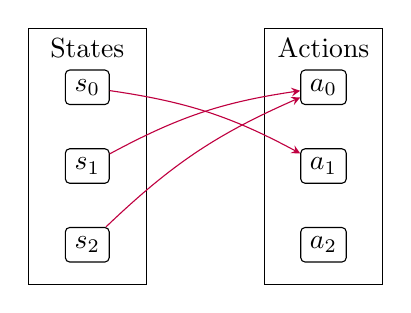
\begin{tikzpicture}
    \node[draw,rectangle,rounded corners=.55mm] (s0) at (0, 0) {$s_0$};
    \node[draw,rectangle,rounded corners=.55mm] (s1) at (0,-1) {$s_1$};
    \node[draw,rectangle,rounded corners=.55mm] (s2) at (0,-2) {$s_2$};
    \draw (-0.75, -2.5) rectangle (0.75, 0.75);
    \node at (0, 0.5) {States};
    \node[draw,rectangle,rounded corners=.55mm] (a0) at (3, 0) {$a_0$};
    \node[draw,rectangle,rounded corners=.55mm] (a1) at (3,-1) {$a_1$};
    \node[draw,rectangle,rounded corners=.55mm] (a2) at (3,-2) {$a_2$};
    \draw (2.25, -2.5) rectangle (3.75, 0.75);
    \node at (3, 0.5) {Actions};
    \path[-stealth,purple] (s0) edge[bend left=10] (a1);
    \path[-stealth,purple] (s1) edge[bend left=10] (a0);
    \path[-stealth,purple] (s2) edge[bend left=10] (a0);
  \end{tikzpicture}
\end{document}